\scanpage{47}
% archive sheet number: 46
\diagram{\resizebox{\linewidth}{!}{\begin{tikzcd}[ampersand replacement=\&,row sep=small,column sep=large]
X_n=\widehat{\mathrm{Spec}}\,k[x_n]\arrow[dd] \& \deleted{\unsure{x_n=}}x_{\unsure{m|n}}^{n}=x_1\\
(\vphantom{\dfrac11} \& \left)\vphantom{\dfrac11}\right.\ \boxed{\begin{array}{ccc}
n&\left\{\begin{array}{c}1\\1\\ \vdots\\1\end{array}\right.&n\end{array}}\ \bigg)\\
X_1=\widehat{\mathrm{Spec}}\,k[x_1=\deleted{\unsure{\zeta}}z]\arrow[dd] \&\\
(\vphantom{\dfrac11} \& \bigg)\ \boxed{\begin{array}{ccc}
\raisebox{-.5ex}{$2$}&\raisebox{-.5ex}{$2$}&1\\&&1\end{array}}\ \bigg)\\
X_0=\widehat{\mathrm{Spec}}\,k[\deleted{\unsure{x}}u] \&
\deleted{\unsure{x}}u=\frac12-\frac14(\deleted{\unsure{x}}z+\deleted{\unsure{x}}z^{-1})
\end{tikzcd}}}

\figure{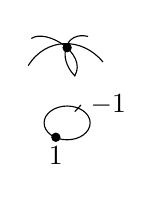
\begin{tikzpicture}[scale=.65]
\draw (-.7,1.1) .. controls (-.4,1.3) and (.4,.8) .. (.15,.37) .. controls (-.2,.72) and (-.04,1.25) .. (.41,1.14);
\draw (-.76,.57) .. controls (-.41,1.13) and (.3,1.13) .. (.7,.64);
\fill (0,.92) circle (2.6pt);
\draw (0,-.55) ellipse (.45 and .33);
\fill (-.22,-.83) circle (2.6pt) node[below] {$1$};
\draw (.15,-.33)--(.27,-.2) node[right] {$-1$};
\end{tikzpicture}}

ramification en dessous des p\textsuperscript{ts} $0,\infty$ (où la ramification est $n$)

p\textsuperscript{ts} de ramification en haut : $0,\infty$

ramification au dessus de

\[
\begin{aligned}
0&\ \deleted{\unsure{\infty\ \text{en haut}}\ (\unsure{\text{pt en dessus}|\text{pts en dessus}}}\inserted{(z=1,\ \text{ramification }2)}\\
1&\ \deleted{\unsure{\text{idem}}}\ (z=-1,\ \text{ramification }2)\\
\infty&\ (0\text{ et }\infty\ \text{ramification }1)
\end{aligned}
\]

\[
\mathbb{D}_\infty=(\mathbb{Z}_{/2})\mathbin{\underset{1/2}{\cdot}}\mu_\infty
\]

\diagram{\resizebox{\linewidth}{!}{\begin{tikzcd}[ampersand replacement=\&,column sep=small,row sep=large]
{\overset{0}{\bullet}\,(n)}\arrow[d] \& \& {\bullet\,\infty\,(n)}\arrow[d] \& {\bullet\,1\ (1)}\arrow[d,"{n\ \text{fois}}" {description,draw,ellipse,inner sep=1pt}] \& {\deleted{\unsure{-1}\ (1)}}\arrow[d,"{\deleted{\diagdown\!\diagdown}}" description] \& \\
0\ (1)\arrow[dr] \& \& \infty\ (1)\arrow[dl,dash] \& 1\ (2)\arrow[d,dash] \& {-1\ \deleted{\unsure{4\,(2)|4\ \text{fois}}}\ (2)}\arrow[d] \& \text{$n$ pair}\\
\& {\bullet\,\infty} \& \& 0 \& 1
\end{tikzcd}}}

\diagram{\begin{tikzcd}[ampersand replacement=\&,column sep=small,row sep=small]
\& \& \bullet\;\infty_1\ (1)\\
\overset{\bullet}{0\,(2)}\&\overset{\bullet}{1\,(2)}\&\bullet\;\infty_2\ (1)\\
\overset{\circ}{0}\&\overset{\cdot}{1}\&\overset{\cdot}{\infty}
\end{tikzcd}}

\figure{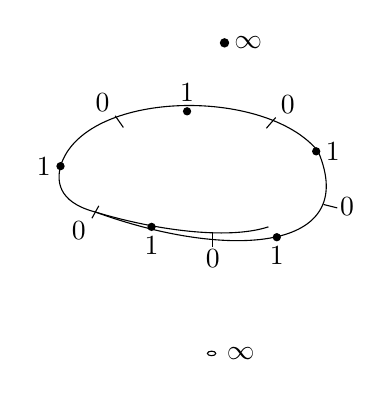
\begin{tikzpicture}[x=.82cm,y=.82cm]
\draw (-2,0) .. controls (-1.64,1.18) and (1.17,1.24) .. (1.99,.23) .. controls (2.65,-1.33) and (.6,-1.46) .. (-1.46,-.71) .. controls (-2.07,-.55) and (-2.05,-.2) .. (-2,0);
\draw[thin] (-1.46,-.71) .. controls (-.57,-.98) and (.57,-1.15) .. (1.22,-.94);
\foreach \x/\y/\a in {-2/0/left,-.04/.85/above,1.96/.23/right,-.59/-.94/below,1.35/-1.1/below}{\fill (\x,\y) circle (1.5pt) node[\a] {$1$};}
\foreach \x/\y/\a/\r in {-1.09/.69/above left/35,1.26/.67/above right/-41,-1.46/-.71/below left/-29,.36/-1.14/below/0,2.18/-.62/right/76}{\draw[shift={(\x,\y)},rotate=\r] (0,-.11)--(0,.11); \node[\a] at (\x,\y) {$0$};}
\fill (.54,1.91) circle (1.7pt) node[right] {$\infty$};
\draw (.34,-2.9) ellipse (.065 and .035) node[right,xshift=2pt] {$\infty$};
\end{tikzpicture}}

% printed form
% Upside-down typed address label.
\begin{center}\rotatebox{180}{\shortstack[l]{MR LE PROFESSEUR GROTHENDIECK A.\\MATHEMATIQUES\hspace{4cm}5}}\end{center}

